\chapter{The models}
In this chapter we discuss several neural network classifiers and their results on our dataset.
\section{Baseline model}
We decided to start with an adaptation of the \textit{optimal} model's architecture outlined in \cite{blackardDean} and reported in Figure \ref{fig:baselinemodel}. The model is made of 51 input nodes, 120 hidden nodes and seven output nodes (symbolized as 51-120-7) where each layer is fully connected. Both the hidden and output layers utilized the logistic (sigmoid) activation functions:
$$
\sigma(a) = \frac{1}{1 + e^{-a}}
$$
Given the training set size, we picked SGD (Stochastic Gradient Descent) as loss function optimizer, while the loss function is the classic MSE (Mean Squared Error, as in \cite{blackardDean}):
\begin{equation}
\text{MSE} = \frac{1}{n}\sum_{i=1}^{n}(Y_i - Y^{*}_{i})^2
\end{equation}
where $Y_i$ is the vector of the true values of the target, $Y^{*}_{i}$ is the model's prediction and $n$ is the number of samples.
\begin{figure}
	\centering
	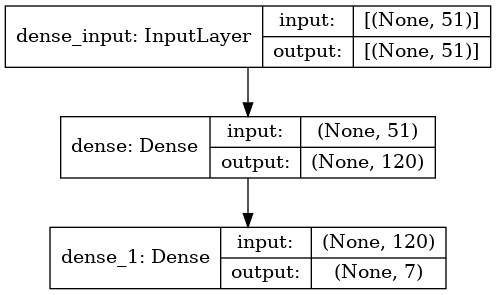
\includegraphics[width=0.7\textwidth]{./TeX_files/img/baselinemodel.png}
	\caption{Baseline model diagram.}
	\label{fig:baselinemodel}
\end{figure}
Setting the learning rate (LR) to $0.05$, the batch size to $128$ and the number of epochs to $200$ the classifier has been trained via a 10-fold cross-validation. The accuracy on the train set and the validation set is shown in Figure \ref{fig:baselinemodelacc} while the losses in Figure \ref{fig:baselinemodelloss}: to smooth the plots, the last metric value for each fold has been taken into account. Given the multi-class nature of the classification task, Figure \ref{fig:confmatheatmap} represent the heat-map rendering of the classification matrix to better convey the information regarding the correctly classified/misclassified samples: it is easy to notice that $532$ samples, of the total $587$ in the test set, belonging to the minority class (Cottonwood/Willow) are correctly classified; $5285$ are misclassified as the minority class but they belong to Ponderosa Pine. Moreover, a good amount of Spruce/Fir samples are correctly classified (this should be expected since this class is one of the majority classes). PARLARE DI PRECISION-RECALL-F1SCORE?
\begin{figure}
	\centering
	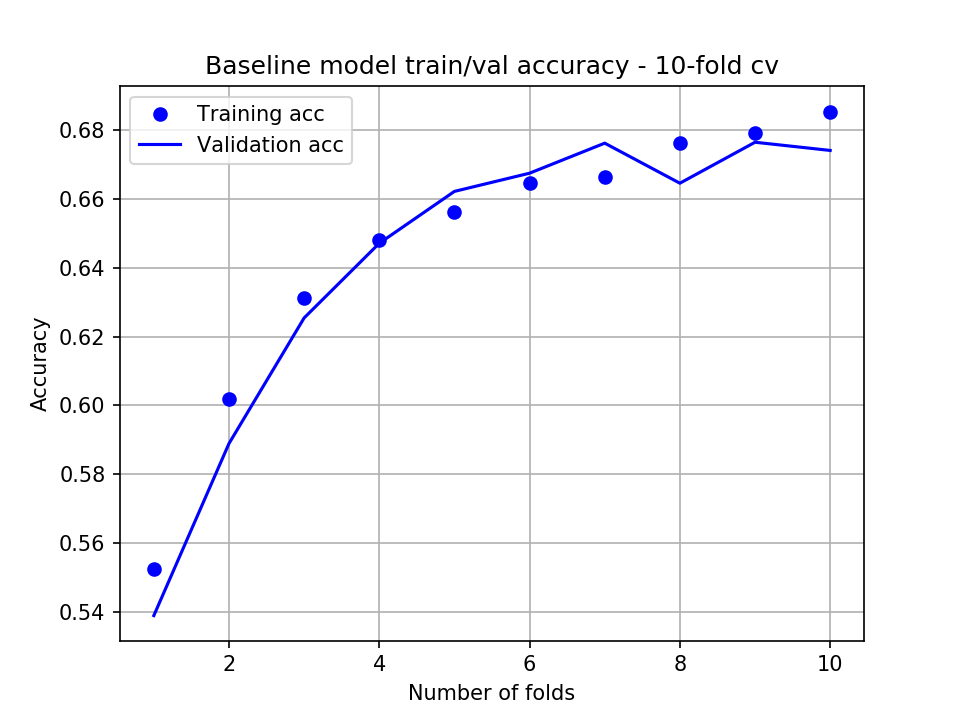
\includegraphics[width=0.7\textwidth]{./TeX_files/img/baselinemodelacc.png}
	\caption{Baseline model accuracy.}
	\label{fig:baselinemodelacc}
\end{figure}
\begin{figure}
	\centering
	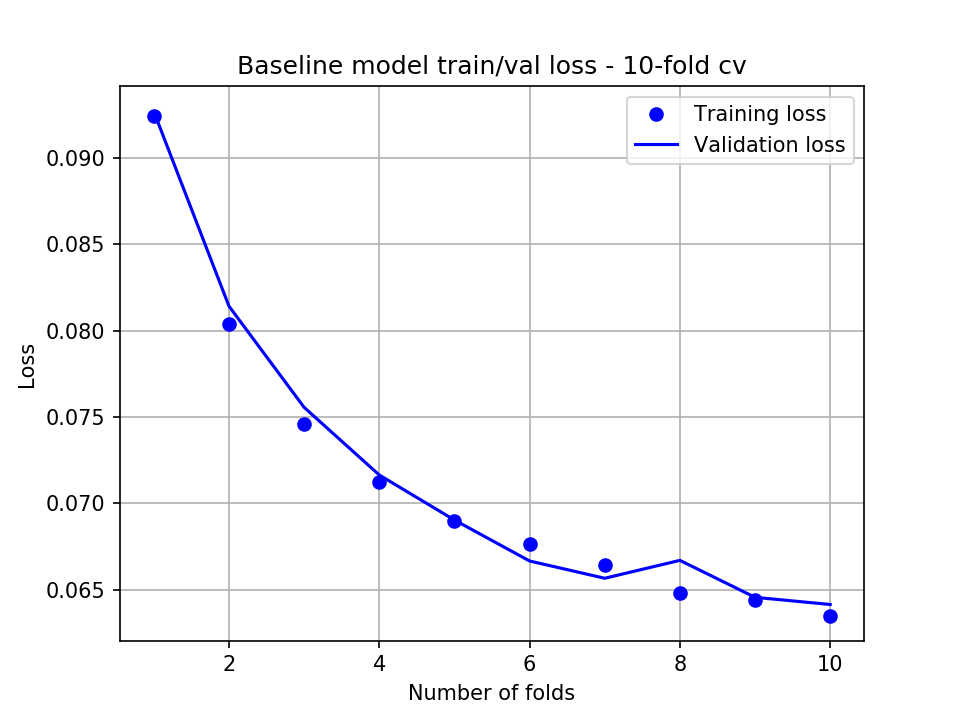
\includegraphics[width=0.7\textwidth]{./TeX_files/img/baselinemodelloss.png}
	\caption{Baseline model losses.}
	\label{fig:baselinemodelloss}
\end{figure}
\begin{figure}
	\centering
	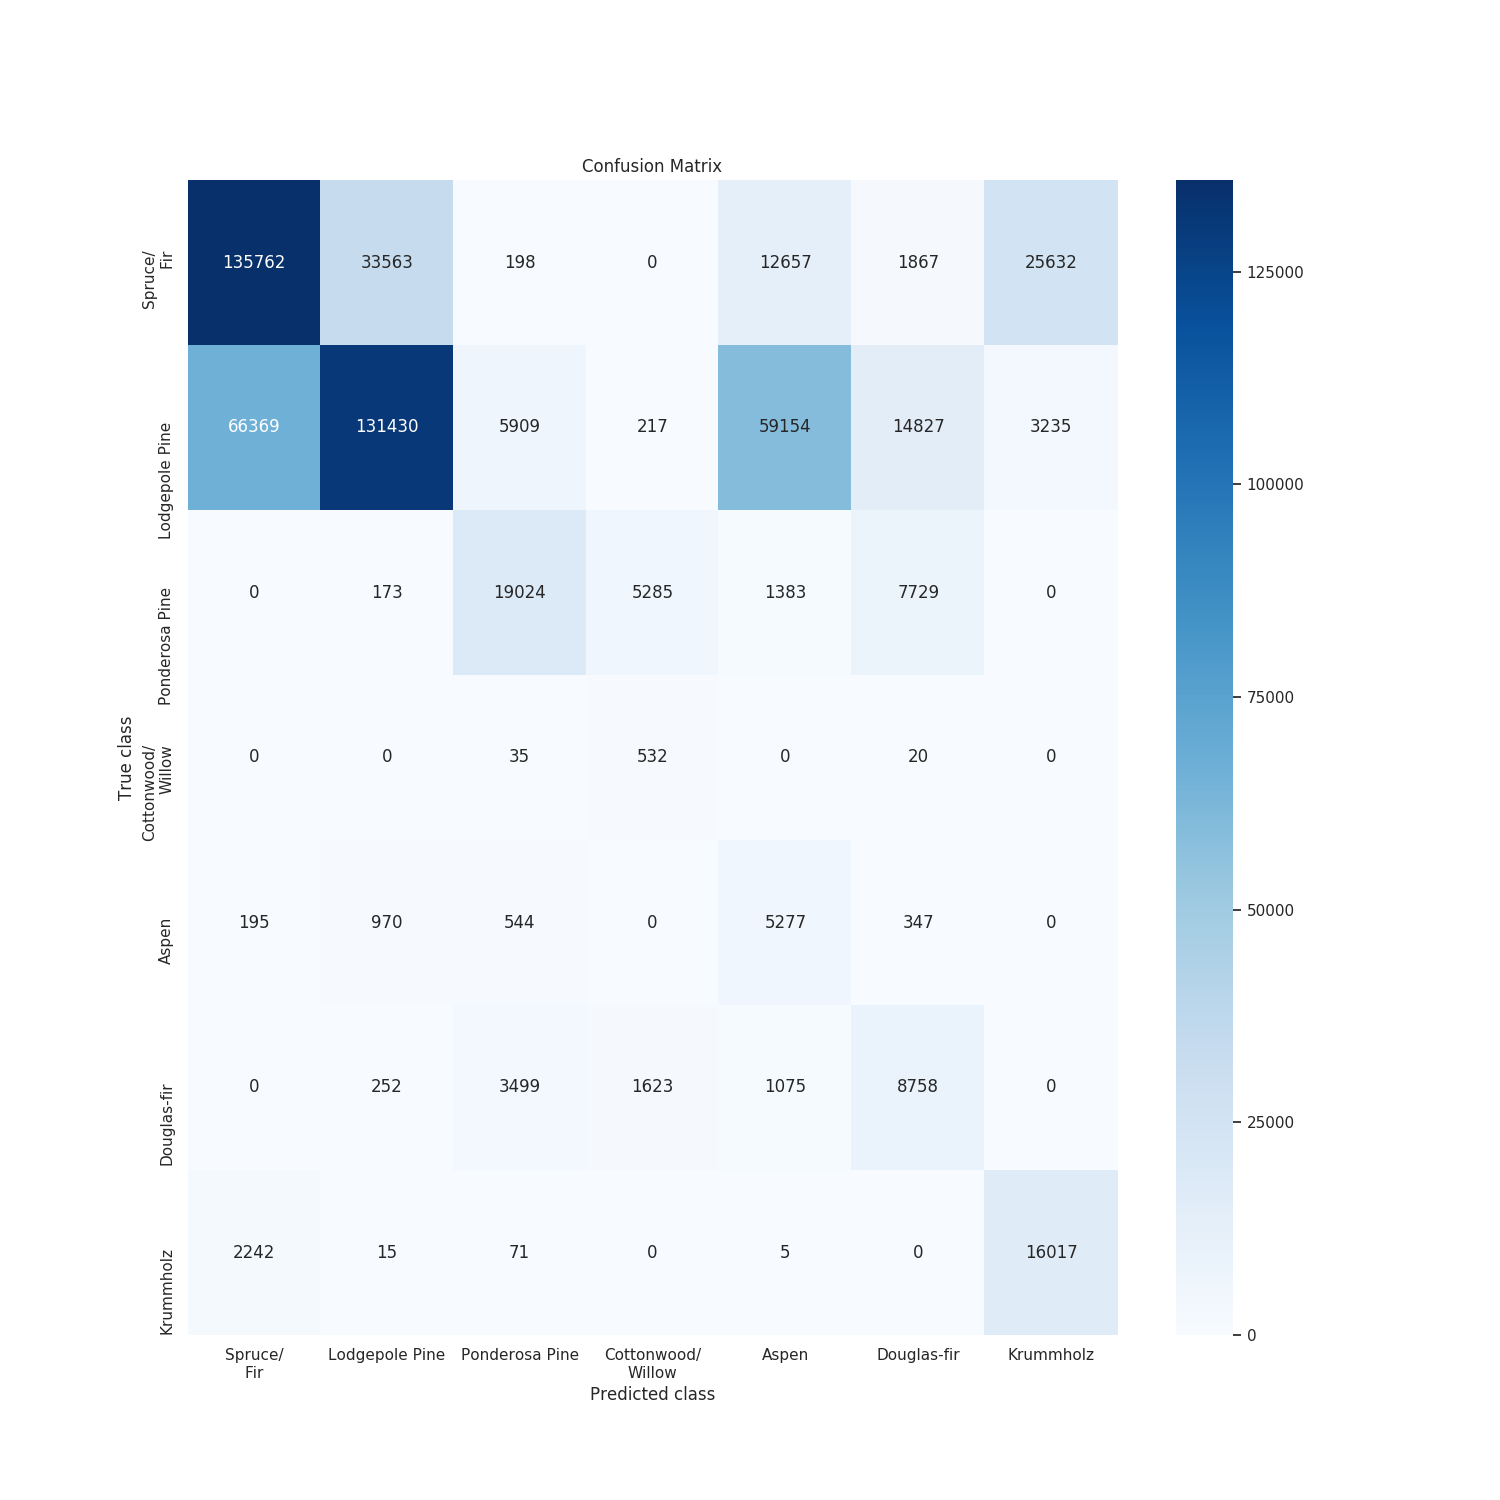
\includegraphics[width=\textwidth]{./TeX_files/img/confmatheatmap.png}
	\caption{Heat-map rendering of the confusion matrix.}
	\label{fig:confmatheatmap}
\end{figure}
\section{Our model}